% Title: Reference modes in ORM2
% Author: Jakob Voß
%
% ORM2 reference mode are only described briefly in Haplin and Morgan (2008) at
% page 85 and 98. This diagram shows what different reference mode kinds hide.
\documentclass{article}
\usepackage{tkz-orm}
\usetikzlibrary{matrix,positioning}
\begin{document}
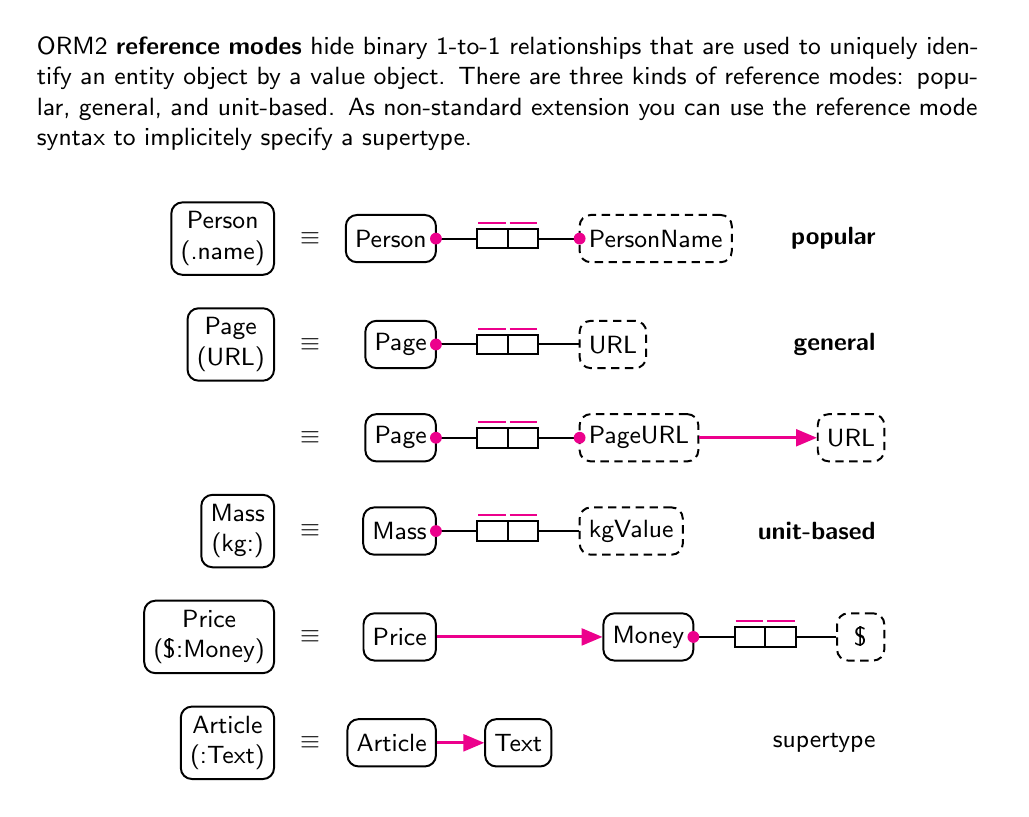
\begin{tikzpicture}[orm]
\node (text) [text width=\textwidth] {
ORM2 {\ormbf reference modes} hide binary 1-to-1 relationships
that are used to uniquely identify an entity object by a value object.
There are three kinds of reference modes: popular, general, and unit-based.
As non-standard extension you can use the reference mode syntax
to implicitely specify a supertype.
};
\matrix[below=of text,column sep=2mm,row sep=4mm,nodes={left}] (M) {
  \entity {Person\\(.name)}; & \node{$\equiv$}; & \entity (Person) {Person}; 
  &[16mm] \value[right] (PersonName) {PersonName}; & \node{\ormbf popular}; \\
  \entity {Page\\(URL)};     & \node{$\equiv$}; & \entity (Page) {Page}; 
  & \value[right] (URL) {URL};               & \node{\ormbf general}; \\
                             & \node{$\equiv$}; & \entity (Page2) {Page}; 
  & \value[right] (PageURL) {PageURL}; & \value (URL2) {URL}; \\
  \entity {Mass\\(kg:)};     & \node{$\equiv$}; & \entity (Mass) {Mass}; 
  & \value[right] (kgValue) {kgValue};           & \node{\ormbf unit-based}; \\
  \entity {Price\\(\$:Money)}; & \node{$\equiv$}; & \entity (Price) {Price}; 
  & & \value (D) {\$}; \\
  \entity {Article\\(:Text)}; & \node{$\equiv$}; & \entity (Article) {Article};
  & & \node {supertype}; \\
};

\draw[both required] (Person) to node[roles,unique,unique=2]{} (PersonName);
\draw[required] (Page) to node[roles,unique,unique=2]{} (URL);

\draw[both required] (Page2) to node[roles,unique,unique=2]{} (PageURL);
\draw[suptype] (PageURL) to (URL2);

\draw[required] (Mass) to node[roles,unique,unique=2]{} (kgValue);

\entity[left=18mm of D] (Money) {Money};
\draw[suptype] (Price) to (Money);
\draw[required] (Money) to node[roles,unique,unique=2]{} (D);

\entity[right=6mm of Article] (Text) {Text};
\draw[suptype] (Article) to (Text);

\end{tikzpicture}
\end{document}